\documentclass[12pt]{standalone}
\usepackage{amsmath,amssymb}
\usepackage{newtxtext,newtxmath}
\usepackage{tikz}
\begin{document}
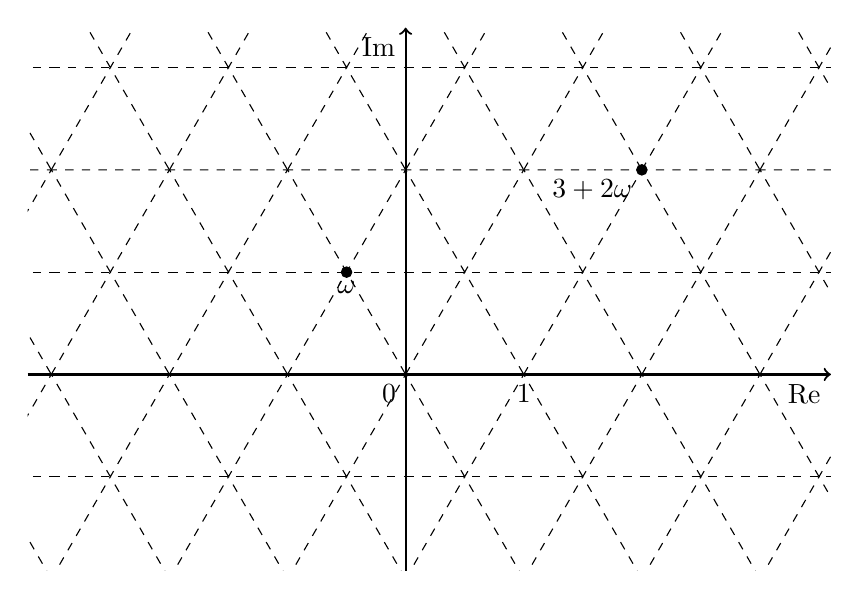
\begin{tikzpicture}[scale=1.5]
\clip (0.8,1.8) rectangle (7.6,6.4);
\def\nx{10}
\def\ny{4} 
\foreach \j in {0,...,\ny} {
    \foreach \i in {0,...,\nx} {
        \draw[dashed](0:\i)++(90:{(1+2*\j)*sin(60)}) -- ++(1,0);
        \draw[dashed](0:\i)++(60:\j)++(120:\j) -- ++(60:2) 
                        -- ++(-1,0) -- ++(-60:1) -- ++(-60:1);
    }
}
\draw[->,thick] (0.8,3.464) -- (7.6,3.464) node[below left]{Re};
\draw[->,thick] (4,1.8) -- (4,6.4) node[below left]{Im};
\draw (4,3.464) node[below left]{$0$};
\draw (5,3.464) node[below]{$1$};
\draw[fill=black] (3.5,4.33) circle (1.25pt) node[below]{$\omega$};
\draw[fill=black] (6,5.196) circle (1.25pt) node[below left]{$3+2\omega$};
\end{tikzpicture}
\end{document}